%!TEX root = ../main.tex

\chapter{Experiments and Analyses}
\label{chp:experiments}

\section{Alarms Report use case}
To evaluate the overall system performance, we focused on reproducing a report that the company has routinely generated and analyzed. By doing so, we were able to directly compare the new \ac{BI} approach with existing processes, using \ac{AWS} tools to replicate the report generation.

The collection named \texttt{alarm} in MongoDB records all alarms triggered by devices, with each alarm containing fields such as the device ID, alarm code, activation timestamp, termination timestamp, and other optional details. The required output for this report is a pivot table: a format used to summarize, analyze, and reorganize data by grouping it across specific dimensions. In this case, the rows represent different devices, while the columns include device details (serial number, model code, family, range, and version) and all potential alarm codes. For each alarm code, we need the total count of occurrences from the past week.

To obtain device-specific details like serial number, model code, and family— which are not present in MongoDB's alarm collection— we also needed to reference the \texttt{device} table stored in PostgreSQL.

Previously, this report was generated through a JavaScript script that used the MongoDB driver to access alarm data and the \ac{ORM} “Sequelize” to access PostgreSQL data. The script would create a \ac{CSV} file that was then automatically emailed to key stakeholders. The entire process was managed by an \ac{AWS} Lambda function scheduled for weekly execution.

To reproduce this outcome using the new \ac{BI} system, we required data from both the “alarm” and “device” tables, which are stored in the data lake's curated layer. To link alarm events with device information, we performed a left join between the two tables, aligning each alarm with its respective device information. We explored three possible solutions for executing this join:

\begin{itemize}
    \item \textbf{Data Lake Join in Analytics Layer}: In this approach, we added steps in the Glue job to read the two tables from the curated layer, join them on the device ID, and write the result in the analytics layer using the Iceberg format. For the alarm table, Glue bookmarks ensure that only new data is read, while the device table is read in full each time. Additionally, the column \texttt{uploaded\_at} is updated to allow QuickSight to refresh only new data. Since both the alarm code and device code are labeled: \texttt{code}, one of them was renamed for clarity. This joined table, identified as "alarm\_device" in the \ac{AWS} catalog, is then ready to be imported into QuickSight as a SPICE or Direct Query dataset. This solution is ideal for regularly scheduled analyses, though it requires \ac{AWS} Glue knowledge, making it less accessible for end users.
    
    \item \textbf{QuickSight Dataset Join}: QuickSight allows datasets to be created by joining other datasets through its visual interface. With both “alarm” and “device” as source datasets, users can create a joined dataset in QuickSight. This approach requires both the source and joined datasets to be in SPICE mode. When the analysis is recurring, daily incremental refreshes are necessary for each dataset, with the joined dataset refreshed last. This solution is more user-friendly and accessible for non-technical users who may need quick analyses, though it incurs storage costs for three SPICE datasets, making it unsuitable for large tables.

    \item \textbf{Athena Join and View Creation}: For users preferring QuickSight's Direct Query mode, the join can be executed in Athena by creating a view: a saved query that functions as a virtual table. This view can then be registered in the \ac{AWS} catalog and used in QuickSight without requiring data refreshes, as queries are executed live.
\end{itemize}

For this use case, the first solution was selected, as it best supports recurrent analyses with frequently updated data. After creating the joined dataset, further preparation was necessary to ensure all fields were analysis-ready. Device details like family, range, and version are embedded within the model code, which is a 14-character alphanumeric string. Specifically, the third character of the model code identifies the family and range, while the twelfth character denotes the version. A calculated field was created for each missing attribute, re-implementing the existing company function to derive these values from the model code directly within QuickSight.

\begin{lstlisting}[caption={Family calculated field}]
ifelse(substring(split({code},'-',1),4,1)='L','MIND.Maps BIG',
substring(split({code},'-',1),3,1)='V','MIND.Maps',
substring(split({code},'-',1),3,1)='B','MIND.Maps',
substring(split({code},'-',1),3,1)='C','MIND.Maps Compact',
substring(split({code},'-',1),3,1)='F','SHOP.Pro',
substring(split({code},'-',1),3,1)='E','Evereo',
substring(split({code},'-',1),3,1)='S','SPEED.Pro',
substring(split({code},'-',1),3,1)='D','Digital.ID',
substring(split({code},'-',1),3,1)='L','Digital.ID',
substring(split({code},'-',1),3,1)='P','Digital.ID',
'')
\end{lstlisting}

Once the dataset was fully prepared, we developed the report using a pivot table with the following configuration: device ID, serial, device code, family, range, and version as rows; alarm codes as columns; and the alarm code counts as values. A filter was applied to the alarm activation date, defaulted to "Last 7 days." The layout was refined to fill the view window, with conditional formatting applied to highlight cells with alarm counts over 50 in orange and over 100 in red.

The resulting analysis was published as an interactive dashboard (shown in Figure \ref{fig:alarmreportquick}) shared with stakeholders, allowing them to adjust the alarm activation date filter to specific relative or absolute periods. With the large number of columns and rows, only visible portions of the table are loaded initially, optimizing performance and accessibility. This setup allows stakeholders to access daily-updated data and view historical data on demand, eliminating the need for weekly emails and file downloads.

\begin{figure}[H]
    \centering
    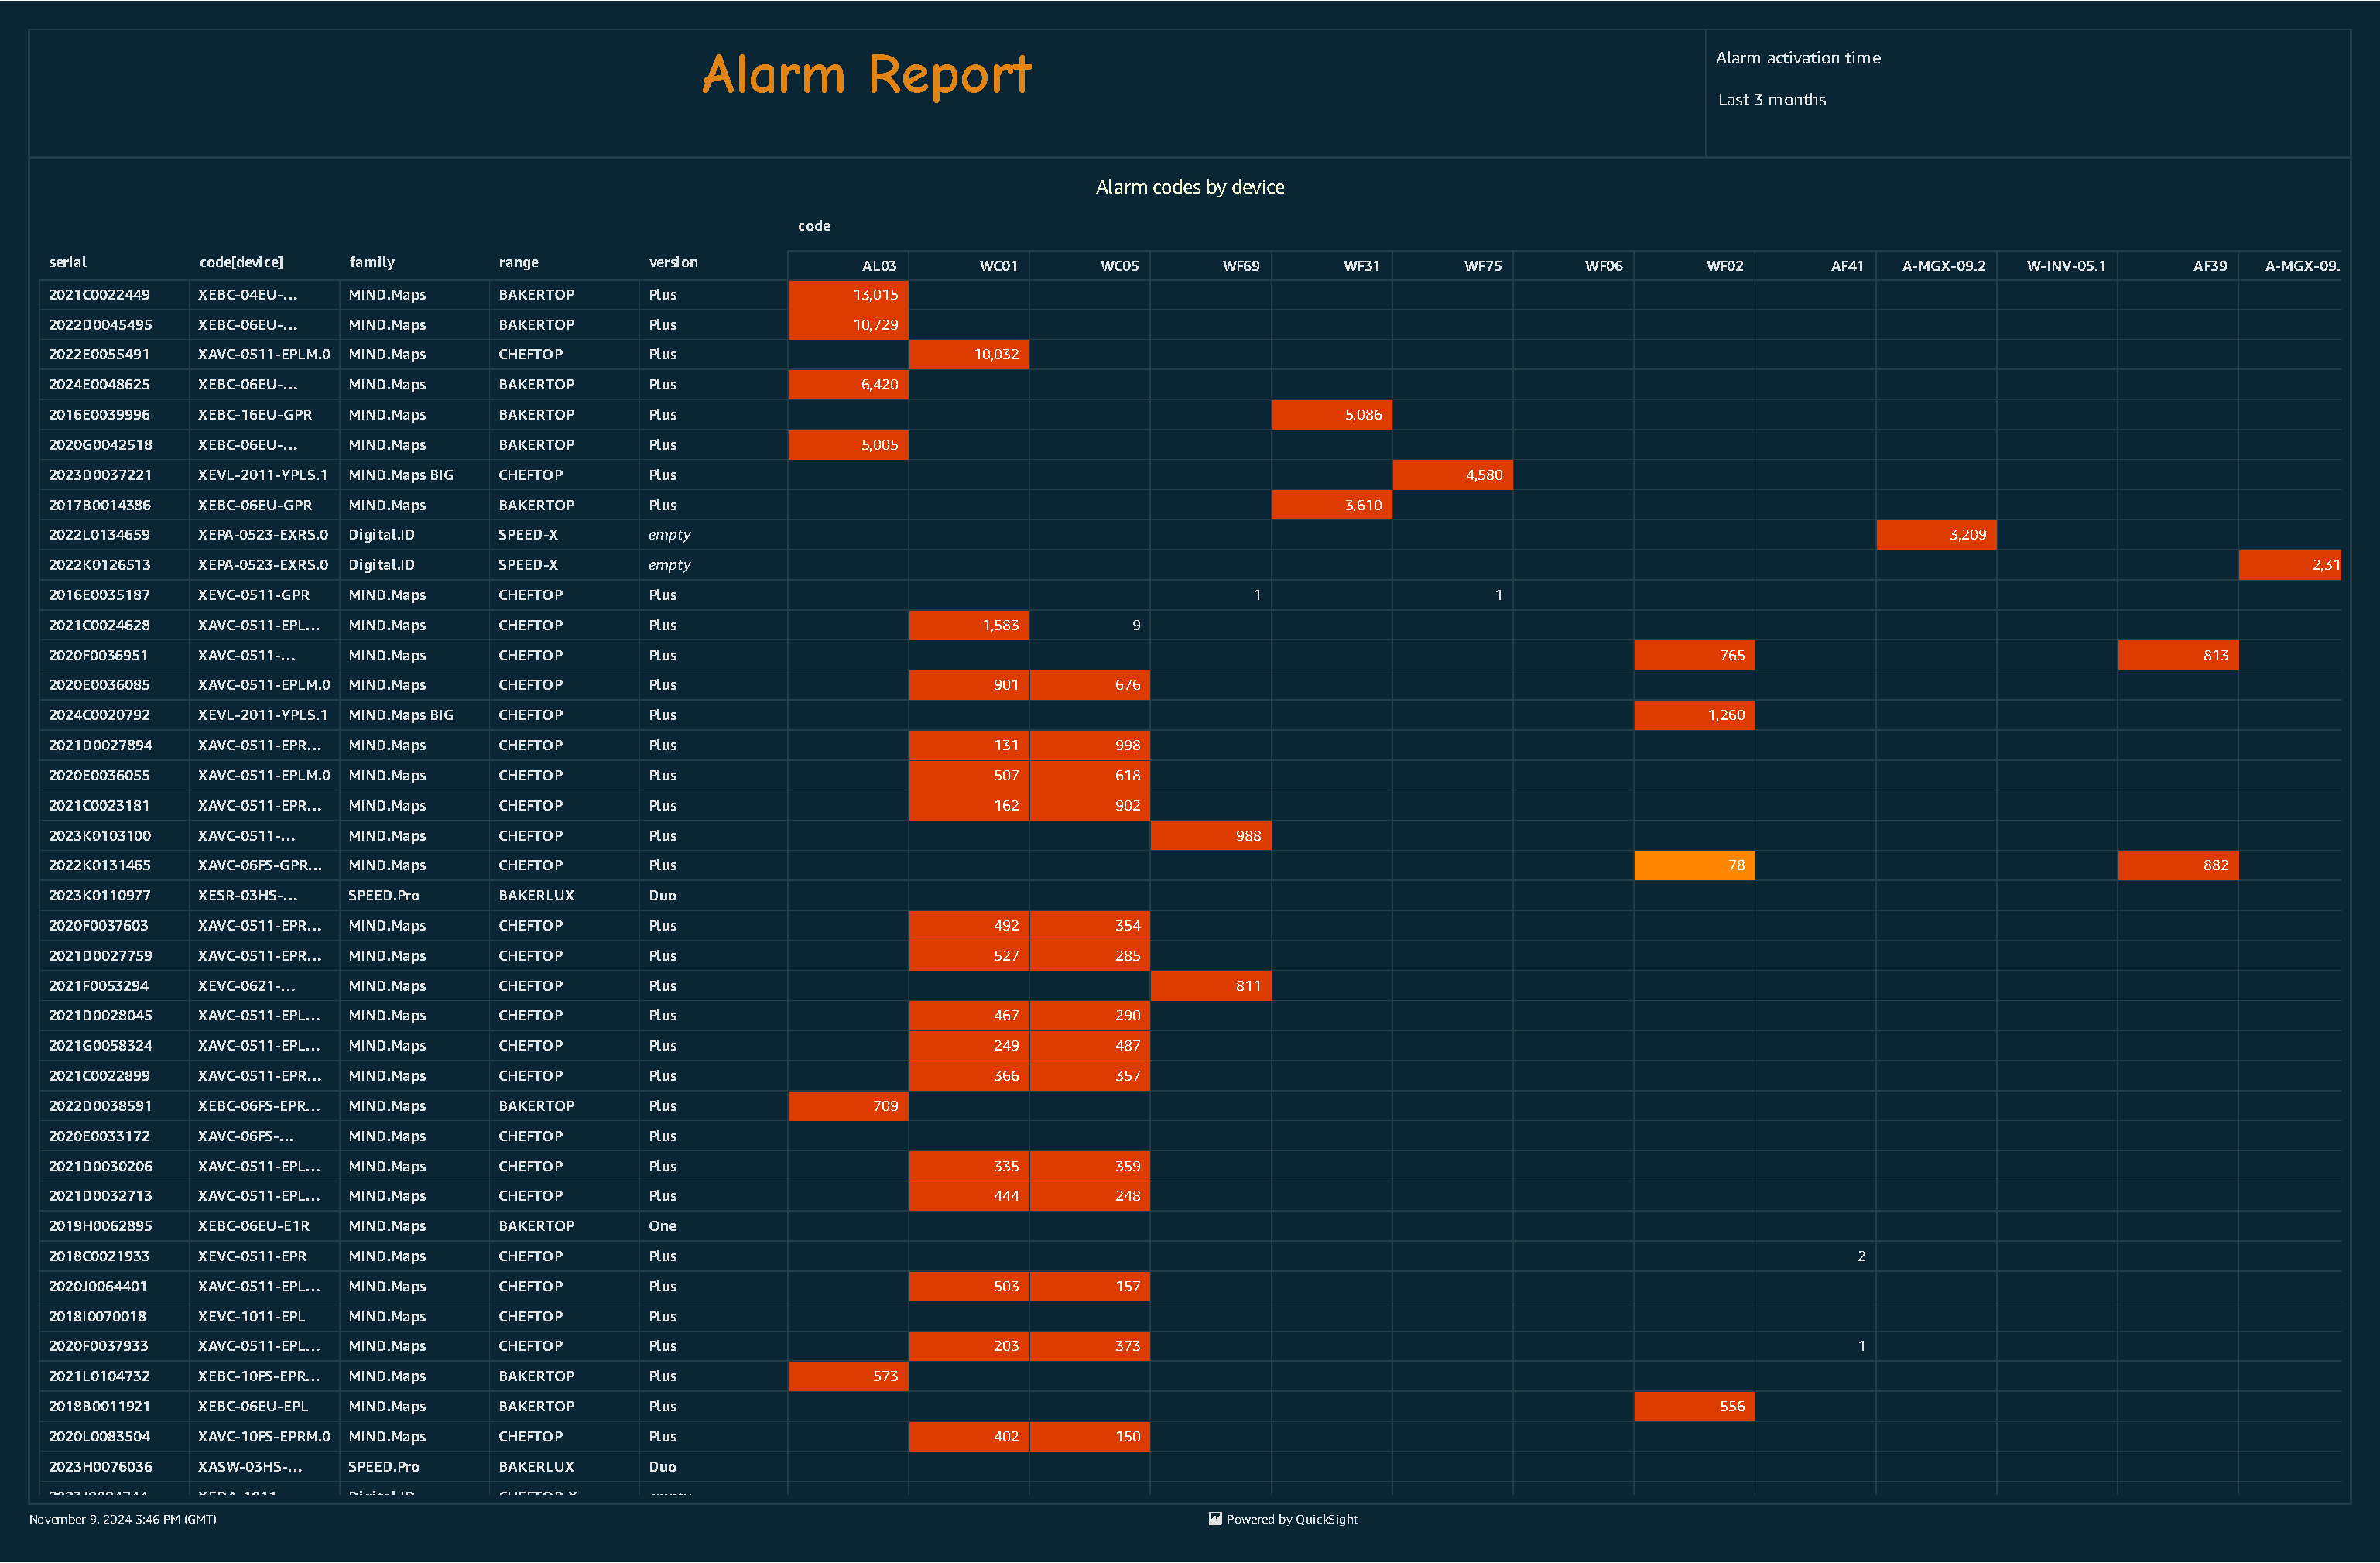
\includegraphics[width=1\textwidth]{res/alarm_report.pdf}
    \caption{Alarm Report from Quicksight}
    \label{fig:alarmreportquick}
\end{figure}

Finally, generative AI was tested by creating a topic based on this dataset. It was necessary to define the scope of the questions, selecting and structuring the relevant data in order to narrow the field of questions that users can ask and make the answers more precise. Through a configuration process, it was possible to enrich the topic with synonyms and phrases commonly used to describe the various data fields. This allows QuickSight Q to recognise different formulations of the same question and still answer correctly.

\section{Partitioning Strategy}
\label{sec:partitioningstrategy}
The following experiment evaluates temporal partitioning strategies for the \textit{mongodb} tables, comparing different levels of time granularity: no time-based partitioning, partitioning by year, and partitioning by month. Specifically, the \texttt{events} table was used for this test, which keeps track of all events occurring in the ovens; examples of frequent events are: door opening/closing, magnetron hour reset, dirt reset, etc. This evaluation aims to identify the impact of each strategy on query performance in terms of execution time and scanned data volume. In all cases, the data is firstly partitioned by device. Then, the analysis explores how adding various levels of time-based partitioning interacts with device-based partitioning, helping to identify the most efficient approach for complex queries involving both device ID and time filters.

Three types of queries were used for each partitioning strategy: a generic time filter (one year and one month), a filter by year, and a filter by month.
\begin{lstlisting}[language=SQL, caption={SQL Queries used for Execution Time and Data Scanning Analysis}]
Generic Filter: 
SELECT * FROM "mongodb"."events" 
WHERE idDevice BETWEEN 1000 AND 5000 AND 
ts BETWEEN TIMESTAMP '2023-01-01' AND TIMESTAMP '2024-01-31';

Year Filter: 
SELECT * FROM "mongodb"."events" 
WHERE idDevice BETWEEN 1000 AND 5000 AND 
ts BETWEEN TIMESTAMP '2023-01-01' AND TIMESTAMP '2023-12-31';

Month Filter: 
SELECT * FROM "mongodb"."events" 
WHERE idDevice BETWEEN 1000 AND 5000 AND 
ts BETWEEN TIMESTAMP '2023-01-01' AND TIMESTAMP '2023-01-31';
\end{lstlisting}

% Grafico dei Tempi di Esecuzione
\begin{figure}[h!]
    \centering
    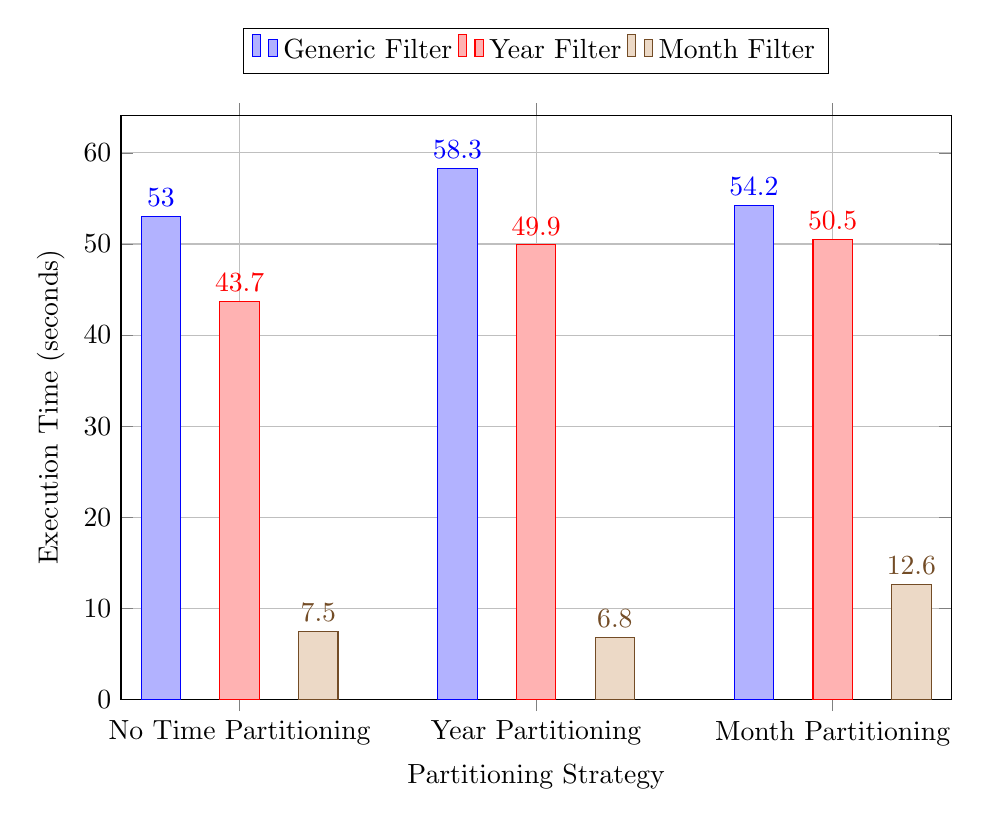
\begin{tikzpicture}
    \begin{axis}[
        ybar=0.5cm,
        bar width=0.5cm,
        width=\textwidth,
        height=9cm,
        symbolic x coords={No Time Partitioning, Year Partitioning, Month Partitioning},
        xtick=data,
        ylabel={Execution Time (seconds)},
        xlabel={Partitioning Strategy},
        ymin=0,
        legend style={at={(0.5,1.15)},
            anchor=north,legend columns=-1},
        nodes near coords,
        nodes near coords align={vertical},
        %title={Query Execution Time by Partitioning Strategy for "events" table},
        enlarge x limits=0.2,
        grid=both
    ]
        \addplot coordinates {(No Time Partitioning, 53) (Year Partitioning, 58.3) (Month Partitioning, 54.2)};
        \addplot coordinates {(No Time Partitioning, 43.7) (Year Partitioning, 49.9) (Month Partitioning, 50.5)};
        \addplot coordinates {(No Time Partitioning, 7.5) (Year Partitioning, 6.8) (Month Partitioning, 12.6)};
        \legend{Generic Filter, Year Filter, Month Filter}
    \end{axis}
    \end{tikzpicture}
    \caption{Query Execution Time by Partitioning Strategy for the \texttt{events} table}
    \label{fig:eventsex}
\end{figure}

The execution time results, displayed in Figure \ref{fig:eventsex}, reveal some unexpected insights. Specifically, the queries on the non-partitioned table exhibit faster performance compared to the year- and month-partitioned tables. For instance, the generic filter query on the non-partitioned table completes in 53 seconds, compared to 58.3 seconds on the year-partitioned table and 54.2 seconds on the month-partitioned table. A similar trend is observed for year-specific and month-specific filters. This counterintuitive outcome can be attributed to the computational overhead of scanning partitions and managing the complexity of partitioned structures. Firstly, when data is partitioned, additional overhead arises from managing partition metadata, which can slow down query processing. Furthermore, partitioning the data into multiple files necessitates more \ac{I/O} operations, as the database engine must access several files to retrieve the relevant data. Consequently, partitioning does not guarantee faster execution for all types of queries.

%However, it is important to note that while non-partitioned tables may provide shorter execution times for these scenarios, this is not a one-size-fits-all solution. In cases where more selective filtering is applied, partitioning by specific keys could lead to substantial performance improvements by avoiding the need to scan irrelevant data. Thus, the optimal partitioning strategy is highly dependent on the expected query patterns.

% Grafico dei Dati Scansionati
\begin{figure}[h!]
    \centering
    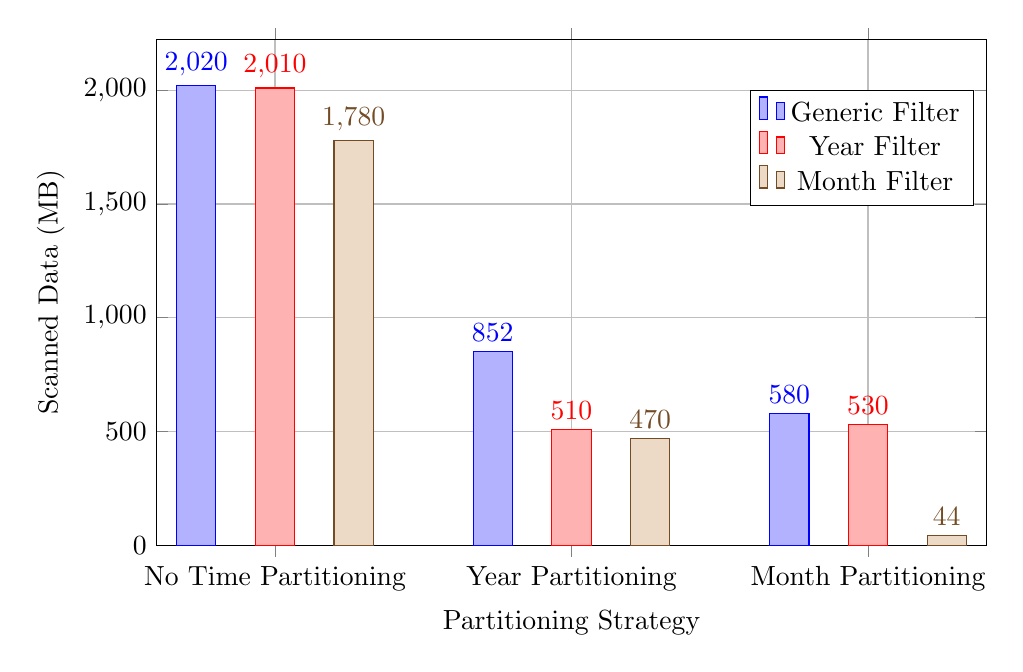
\begin{tikzpicture}
    \begin{axis}[
        ybar=0.5cm,
        bar width=0.5cm,
        width=\textwidth,
        height=8cm,
        symbolic x coords={No Time Partitioning, Year Partitioning, Month Partitioning},
        xtick=data,
        ylabel={Scanned Data (MB)},
        xlabel={Partitioning Strategy},
        ymin=0,
        legend style={at={(0.85,0.9)},
            anchor=north,legend columns=1},
        nodes near coords,
        nodes near coords align={vertical},
        %title={Scanned Data by Partitioning Strategy for "events" table},
        enlarge x limits=0.2,
        grid=both
    ]
        \addplot coordinates {(No Time Partitioning, 2020) (Year Partitioning, 852) (Month Partitioning, 580)};
        \addplot coordinates {(No Time Partitioning, 2010) (Year Partitioning, 510) (Month Partitioning, 530)};
        \addplot coordinates {(No Time Partitioning, 1780) (Year Partitioning, 470) (Month Partitioning, 44)};
        \legend{Generic Filter, Year Filter, Month Filter}
    \end{axis}
    \end{tikzpicture}
    \caption{Scanned Data by Partitioning Strategy for the \texttt{events} table}
    \label{fig:eventscan}
\end{figure}

The data scanned, as shown in Figure \ref{fig:eventscan}, illustrates the effectiveness of partitioning in reducing the volume of data processed for targeted queries. For instance, the month-specific filter in the month-partitioned table scans only 44 MB, compared to 1,780 MB in the non-partitioned table and 470 MB in the year-partitioned table. This reduction demonstrates the value of partitioning in limiting data scans when filters closely match the partitioning strategy. Conversely, without partitioning, the table must scan a substantially larger amount of data, as all records are treated as a single, unstructured set. 

The findings underscore the importance of selecting appropriate partitioning strategies based on the nature of the queries executed and the underlying data characteristics. While smaller partitioning intervals can enhance data efficiency and significantly reduce the volume of scanned data, they may also introduce a slight increase in execution time due to the necessity of additional metadata reads and higher \ac{I/O} access counts. Therefore, a balance must be found between minimizing scanned data and optimizing execution times to achieve the best performance in data querying and processing.

\subsubsection{Partitioning Strategy Results on "sd\_variables" Table}
The same test performed with ‘events’ was re-executed on the table \\\texttt{sd\_variables} to confirm the results obtained.
"sd\_variables" contains about 8 times fewer documents than “events”, but these are much heavier (see table \ref{tab:sizes}). Specifically, "sd\_variables" contains the \ac{IoT} values generated by Digital ID devices, i.e. the highest oven range produced by Unox.

% Grafico dei Tempi di Esecuzione e Dati Scansionati
\begin{figure}[h!]
    \centering
    % Inizio del primo grafico
    \begin{minipage}{0.48\textwidth}
        \centering
        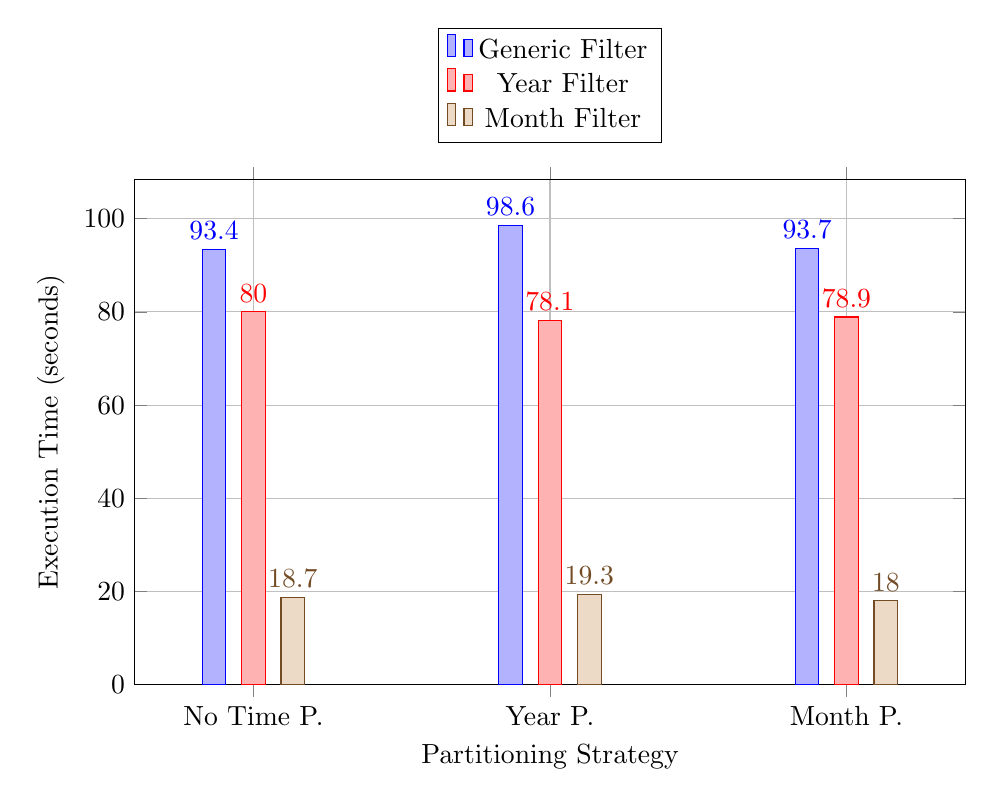
\begin{tikzpicture}
        \begin{axis}[
            ybar=0.2cm,
            bar width=0.3cm,
            width=\textwidth,
            height=8cm,
            symbolic x coords={No Time P., Year P., Month P.},
            xtick=data,
            ylabel={Execution Time (seconds)},
            xlabel={Partitioning Strategy},
            ymin=0,
            legend style={at={(0.5,1.3)},
                anchor=north,legend columns=1},
            nodes near coords,
            nodes near coords align={vertical},
            enlarge x limits=0.2,
            grid=both
        ]
            \addplot coordinates {(No Time P., 93.4) (Year P., 98.6) (Month P., 93.7)};
            \addplot coordinates {(No Time P., 80) (Year P., 78.1) (Month P., 78.9)};
            \addplot coordinates {(No Time P., 18.7) (Year P., 19.3) (Month P., 18)};
            \legend{Generic Filter, Year Filter, Month Filter}
        \end{axis}
        \end{tikzpicture}
    \end{minipage}%
    \hfill
    % Inizio del secondo grafico
    \begin{minipage}{0.48\textwidth}
        \centering
        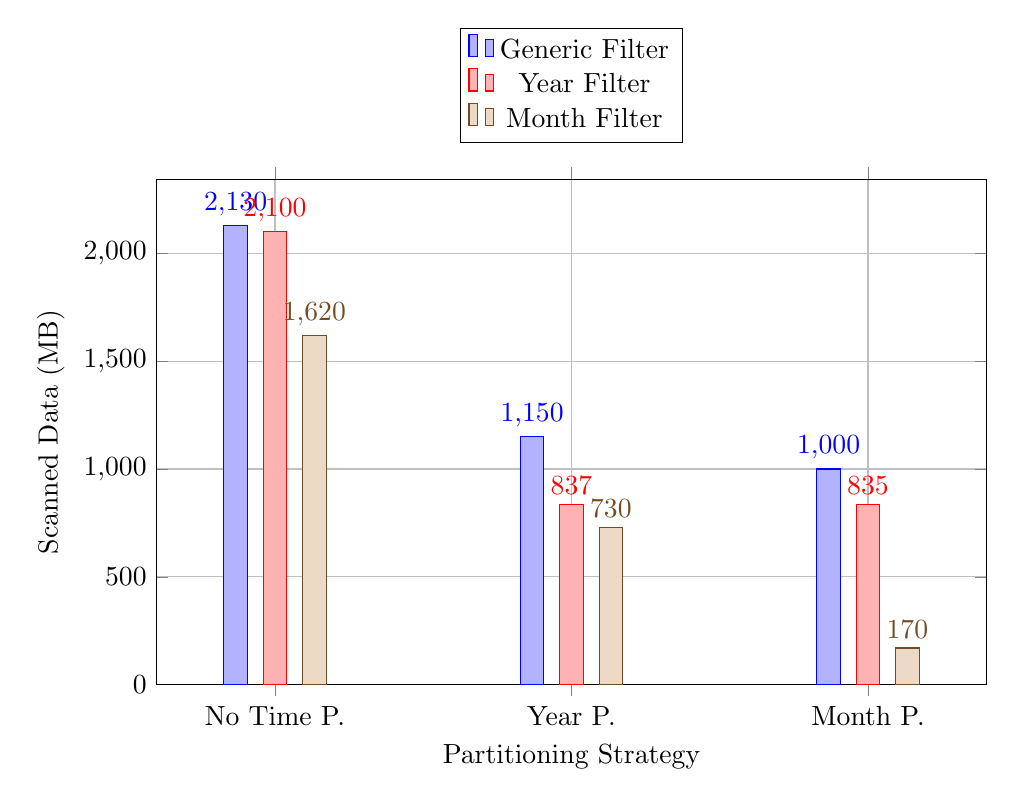
\begin{tikzpicture}
        \begin{axis}[
            ybar=0.2cm,
            bar width=0.3cm,
            width=\textwidth,
            height=8cm,
            symbolic x coords={No Time P., Year P., Month P.},
            xtick=data,
            ylabel={Scanned Data (MB)},
            xlabel={Partitioning Strategy},
            ymin=0,
            legend style={at={(0.5,1.3)},
                anchor=north,legend columns=1},
            nodes near coords,
            nodes near coords align={vertical},
            enlarge x limits=0.2,
            grid=both
        ]
            \addplot coordinates {(No Time P., 2130) (Year P., 1150) (Month P., 1000)};
            \addplot coordinates {(No Time P., 2100) (Year P., 837) (Month P., 835)};
            \addplot coordinates {(No Time P., 1620) (Year P., 730) (Month P., 170)};
            \legend{Generic Filter, Year Filter, Month Filter}
        \end{axis}
        \end{tikzpicture}
    \end{minipage}
    % Didascalia comune
    \caption{Query Execution Time and Scanned Data by Partitioning Strategy for \texttt{sd\_variables} table}
    \label{fig:vars}
\end{figure}

As shown in Figure \ref{fig:vars}, execution times for queries on "sd\_variables" display only minor variations across partitioning strategies. In the case of year and month filters, the execution times remain relatively consistent across strategies, with a marginally faster performance for year-based and month-based partitioning compared to no partitioning.

In terms of scanned data, partitioning again shows a clear advantage in limiting the volume of data processed, especially for month-specific queries. For instance, the month-specific query scans only 170 MB in the month-partitioned table, while the no-partition approach scans up to 1,620 MB. These reductions in data scanning are similar to those noted in the "events" table, where finer-grained partitions significantly minimized data read volumes.

Based on these observations and tests, a year-based partitioning strategy has been chosen as an effective compromise. While finer-grained (month-based) partitioning minimizes scanned data, it often results in higher execution times due to the overhead associated with managing more granular partitions. Consequently, year-based partitioning offers a balanced trade-off, achieving acceptable query times while reducing data scans effectively for time-based filters.

\section{Benchmark of the BI System}
This section presents a benchmark comparing query execution times on \ac{AWS} Athena and the original MongoDB data sources. Since Postgres tables contain relatively small amounts of data and are generally not the bottleneck in business analyses, tests focused primarily on MongoDB tables. The queries on the original MongoDB source were executed using Studio 3T, a widely used GUI tool that facilitates query building, performance tuning, and data analysis. Before executing the benchmark, it was crucial to verify data consistency between the DBMSs and the data lake, especially considering frequent daily updates.

To ensure a reliable comparison, five representative queries were executed on both systems, with each query being run seven times on each system to calculate an average execution time. The test queries were executed on the \texttt{end\_of\_prog\_aggregated} table, which contains a moderate number of documents with an average size compared to other tables.

The MongoDB performance is shown in two scenarios: with no optimizations and with optimizations. The available optimizations include:

\begin{itemize}
    \item \textbf{Index Plan for a Query}: MongoDB caches the query execution plan, reducing the need to evaluate which index to use on repeated queries, which helps speed up execution.
    \item \textbf{Index Cached in Memory}: When an index is used, MongoDB caches it in memory, so subsequent queries using the same index can access it faster.
    \item \textbf{Data Cached in Memory}: MongoDB relies on the operating system's memory management system, which caches frequently accessed data. Once a document is read, it stays in memory, significantly reducing access time for future queries that request the same data.
\end{itemize}

The \textit{index} in MongoDB is a data structure that speeds up query execution by enabling fast searching within the data \cite{chopade2020mongodb}. When a query is run for the first time, MongoDB must scan through the dataset and load the necessary index into memory. Once cached, the subsequent executions of the same query are faster, as the data and index reside in memory. Each collection contains at least one index consisting of the \textit{idDevice} and timestamp fields.

Therefore, the first execution of each query requires reading the data and index from the disk and moving them into memory, which takes an enormous amount of time. Moreover, considering the \ac{EC2} instance has only 32 GiB of memory, only a fraction of the datasets/indexes can be cached at any given time, making MongoDB's performance highly dependent on caching.

The following is a brief description of the five test queries executed on both systems:

\begin{itemize}
    \item \textbf{Query 1}: Returns documents generated after January 1, 2024.
    \item \textbf{Query 2}: Groups documents by device and calculates the average energy consumed during cooking for each device.
    \item \textbf{Query 3}: Filters documents with daily cooking time greater than one hour, groups them by device, and calculates the total cooking time, then orders the results by descending cooking time.
    \item \textbf{Query 4}: Groups devices into five cooking times ranges, counts the number of devices in each range, and calculates the average cooking energy for each range, presenting the results in ascending order.
    \item \textbf{Query 5}: Performs a join between the "end\_of\_prog\_aggregated" table and the \texttt{sdata} table (containing device configuration information) based on the device ID.
\end{itemize}

In the first four queries, 5000 devices were filtered to reduce execution time, while in the last query only 500 devices were filtered.
\begin{figure}[H]
    \centering
    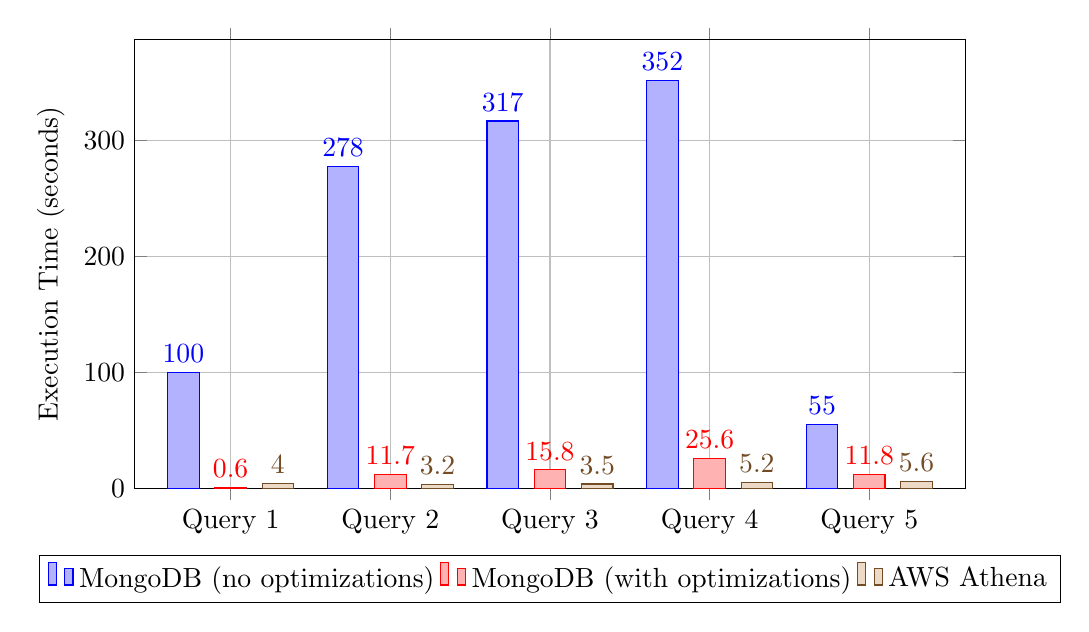
\begin{tikzpicture}
        \begin{axis}[
            ybar=0.2cm,
            bar width=0.4cm,
            width=\textwidth,
            height=0.6\textwidth,
            enlarge x limits=0.15,
            ylabel={Execution Time (seconds)},
            symbolic x coords={Query 1, Query 2, Query 3, Query 4, Query 5},
            xtick=data,
            nodes near coords,
            legend style={at={(0.5,-0.15)}, anchor=north, legend columns=-1},
            ymin=0,
            grid=both
        ]
            \addplot coordinates {(Query 1,100) (Query 2,278) (Query 3,317) (Query 4,352) (Query 5,55)};
            \addplot coordinates {(Query 1,0.6)  (Query 2,11.7)  (Query 3,15.8)  (Query 4,25.6) (Query 5,11.8)};
            \addplot coordinates {(Query 1,4) (Query 2,3.2) (Query 3,3.5) (Query 4,5.2) (Query 5,5.6)};
    
            \legend{MongoDB (no optimizations), MongoDB (with optimizations), AWS Athena}
        \end{axis}
    \end{tikzpicture}
    \caption{Query Execution Time on AWS Athena and MongoDB (optimized and not optimized) for \texttt{end\_of\_prog\_aggregated} table}
    \label{fig:eopaex}
\end{figure}

The results in Figure \ref{fig:eopaex} clearly show the significant performance improvement with optimizations in MongoDB. In the "no optimizations" case, MongoDB's query times are significantly higher, as it must read both the data and indexes from disk. With optimizations enabled, the query times decrease dramatically, as both the data and indexes are cached in memory. However, when comparing MongoDB with \ac{AWS} Athena, it is evident that Athena consistently outperforms MongoDB, even with all optimizations applied.

\ac{AWS} Athena achieves execution times that are 10 to 70 times faster than MongoDB in its non-optimized state, which is the typical case in most business intelligence analyses, as queries are often run on-demand or with low frequency, preventing data and indexes from remaining in memory.

In conclusion, while MongoDB, with proper optimizations, can deliver competitive performance for smaller datasets, Athena outperforms MongoDB in large-scale data processing scenarios, especially when query performance and scalability are crucial.

\section{Cost Estimation}
Once the system had been tested and validated, it was essential to estimate the costs of each \ac{AWS} service utilized. This estimation provides the company with an approximate understanding of the total solution cost. For simplicity, costs were divided into two phases: the bulk load and operational phases. The bulk load represents a one-time expense, while operational costs recur monthly and depend on user activity.

\subsection{Bulk Load Phase Cost Summary}
The following table summarizes the estimated costs for the bulk load phase:

\begin{table}[h]
    \centering
    \begin{tabular}{|p{2.75cm}|p{2.5cm}|p{6.5cm}|p{1.75cm}|}
        \hline
        \textbf{AWS Service} & \textbf{Feature} & \textbf{Description} & \textbf{Cost (\$)} \\ \hline
        \textbf{Lambda} & Elaboration & ((46,000 requests $\times$ 450 s $\times$ 6 GB) - 400,000 GB/s) $\times$ 0.0000166667 USD & 2,063.34 \\ \hline
        \textbf{Glue} & ETL mongo & 5,000 DPU $\times$ 0.42 hours $\times$ 0.29 USD & 604.18 \\ \hline
        & ETL postgres & 20 DPU $\times$ 0.42 hours $\times$ 0.29 USD & 2.43 \\ \hline
        \textbf{S3 (Raw)} & Storage & 2,400 GB $\times$ 0.0245 USD & 58.80 \\ \hline
        & PUT requests & 3,000,000 requests $\times$ 0.0000054 USD & 16.20 \\ \hline
        \textbf{S3 (Curated)} & Storage & 300 GB $\times$ 0.0245 USD & 7.35 \\ \hline
        & PUT requests & 1,000,000 requests $\times$ 0.0000054 USD & 5.40 \\ \hline
        \textbf{S3 (Analytics)} & Storage & 34 GB $\times$ 0.0245 USD & 0.83 \\ \hline
        & PUT requests & 1,000,000 requests $\times$ 0.0000054 USD & 5.40 \\ \hline
        \textbf{RDS} & Instance & 730 hours $\times$ 0.074 USD & 54.02 \\ \hline
        & Storage & 50 GB $\times$ 0.137 USD & 6.85 \\ \hline
        \multicolumn{3}{|l|}{\textbf{Total}} & \textbf{2,824.80} \\ \hline
    \end{tabular}
    \caption{AWS Service Costs for the Bulk Load Phase}
    \label{tab:bulk_load_costs}
\end{table}

In this one-time phase, costs were incurred primarily by Lambda, Glue, \ac{S3}, and \ac{RDS}. Approximately 46,000 Lambda invocations were required to process the initial data load, involving complex orchestration between master and worker functions, each with an estimated average runtime of 7 minutes and memory usage of 6 GB. Glue costs stemmed mainly from the \ac{ETL} processes handling data transformation, especially for MongoDB, which demanded approximately 20 \ac{DPU} per function. The \ac{RDS} instance, slightly overprovisioned for initial testing, could potentially be downsized to reduce costs. Costs for GET requests in \ac{S3} were negligible and thus omitted.

\subsection{Operational Phase Monthly Costs}
\label{sec:operationalcosts}
The table below shows the monthly costs for the system's operational phase:

\begin{table}[h]
    \centering
    \begin{tabular}{|p{2.75cm}|p{2.5cm}|p{6.5cm}|p{1.75cm}|}
        \hline
        \textbf{AWS Service} & \textbf{Feature} & \textbf{Description} & \textbf{Cost (\$)} \\ \hline
        \textbf{Lambda} & Elaboration & ((1,217 requests $\times$ 720 s $\times$ 6 GB) - 400,000 GB/s) $\times$ 0.0000166667 USD & 80.93 \\ \hline
        \textbf{Glue} & ETL mongo curated & 600 DPU $\times$ 0.42 hours $\times$ 0.29 USD & 73.08 \\ \hline
        & ETL postgres & 600 DPU $\times$ 0.1 hours $\times$ 0.29 USD & 17.40 \\ \hline
        & ETL analytics & 600 DPU $\times$ 0.05 hours $\times$ 0.29 USD & 8.70 \\ \hline
        \textbf{S3 (Raw)} & Storage & 2,400 GB $\times$ 0.0245 USD & 58.80 \\ \hline
        & PUT requests & 1,500,000 requests $\times$ 0.0000054 USD & 8.10 \\ \hline
        \textbf{S3 (Curated)} & Storage & 300 GB $\times$ 0.0245 USD & 7.35 \\ \hline
        & PUT requests & 1,500,000 requests $\times$ 0.0000054 USD & 8.10 \\ \hline
        \textbf{S3 (Analytics)} & Storage & 34 GB $\times$ 0.0245 USD & 0.83 \\ \hline
        & PUT requests & 1,000,000 requests $\times$ 0.0000054 USD & 5.40 \\ \hline
        \textbf{Athena} & Queries & 1,521 queries $\times$ 0.009765625 TB $\times$ 5.00 USD & 74.27 \\ \hline
        \textbf{QuickSight} & Readers & 10 Readers $\times$ 3.00 USD & 30.00 \\ \hline
        & Authors & 1 Author $\times$ 24.00 USD & 24.00 \\ \hline
        & SPICE & (100 GB - (10.00 GB $\times$ 1 author)) $\times$ 0.38 USD & 34.20 \\ \hline
        \multicolumn{3}{|l|}{\textbf{Total}} & \textbf{431.16} \\ \hline
    \end{tabular}
    \caption{AWS Service Costs for the Operational Phase (Monthly)}
    \label{tab:operational_costs}
\end{table}

These monthly operational costs are estimated based on an expected daily load of 40 Lambda invocations with a runtime average of 10 minutes each. Glue requires 20 \ac{DPU}s daily for \ac{ETL} processes. Athena costs vary depending on usage but are estimated with a baseline of 50 queries per day, scanning approximately 10 GB of data each. QuickSight includes 10 reader accounts and 1 author account, along with 100 GB of SPICE storage. The estimate does not include the use of generative AI with Quicksight Q, which would require an increase of at least \$275 per month. \ac{RDS} costs are negligible here, as daily upserts are minimal and could be handled by an \ac{RDS} instance with lower performance or by leveraging free \ac{AWS} options.
In summary, the system has an initial cost of approximately 2800 USD for the \textit{bulk load} phase and for the ongoing \textit{operational} phase, the estimated monthly cost is around 430 USD. Operational expenses vary a lot based on actual system utilization by users.